\documentclass{beamer}
\usetheme{Madrid}
\usecolortheme{whale}

\usepackage{appendixnumberbeamer}
\usepackage{multimedia}
\usepackage{braket}
\usepackage{array}
\definecolor{mypurple}{RGB}{255,0,255}

\newcommand{\abs}[1]{\left\lvert #1 \right\rvert}
\graphicspath{ {Graphics/}  }
\setbeamerfont{caption}{size=\scriptsize}

\title[Scalable Trapped Ion Quantum Computing]{Scalable Trapped Ion Quantum Computing using Multiple Ion Species}
\subtitle{Barium and Ytterbium Ion Chains for Quantum Computation}
\author[J. Wright]{John Wright}
\institute[UW] {
	Department of Physics \\
	University of Washington
}
\date[June 2013]{June 4, 2013}

\begin{document}

\begin{frame}[plain]
\titlepage
\end{frame}

\section{MUSIQC}
\begin{frame}{MUSIQC - Introduction}
Modular Universal Scalable Ion-Trap Quantum Computer
\begin{itemize}
	\item Final deliverable planned to have 80 qubits
	\item Plan to have largest possible ion chains in each trap %
		and scale further by linking ions via radiated photons
\end{itemize}
\centerline{\includegraphics[height=0.38\textheight]{MUSIQC-plan}}
\let\thefootnote\relax\footnote[frame]{C.Monroe, et al, 2012, arXiv:1208.0391}
\end{frame}

\begin{frame}{MUSIQC - Using Multiple Ion Species}
Within the MUSIQC architecture we plan to have local motional gates between ions in the same trap and remote entanglement via photons to couple multiple traps
\begin{itemize}
	\item Light from Barium's cooling transition (493nm) is easily transferred long distances via optical fiber
	\item Yb-171 has long lived hyperfine states that can easily be frequency initialized and used for motional gates
	\item By separating these tasks to different species the possibility for crosstalk is reduced
\end{itemize}
\end{frame}

\section[BaYb]{Barium-Ytterbium System}
\begin{frame}{Trapping Barium and Ytterbium}
\begin{columns}
	\begin{column}{0.4\textwidth}
		\centerline{\includegraphics[width=0.9\textwidth]%
			{BaYb}}
	\end{column}
	\begin{column}{0.6\textwidth}
		\begin{itemize}
			\item Crystal contains two cooled, bright Ba ions and one dark Yb ion
			\item Secular frequency shift has been measured to confirm the presence of Yb
			\item Yb ions are loaded via charge exchange with trapped Ba ions
			\item Need to further study cooling efficiency of long mixed species chains
		\end{itemize}
	\end{column}
\end{columns}
\end{frame}

\begin{frame}{Mixed Species Normal Modes}
Trapping different mass ions in the same potential causes the normal
modes of the different species to decouple.
\par\medskip
\begin{center}\begin{tabular*}{1.0\textwidth}{@{\extracolsep{\fill}} lr}
	\includegraphics[width=0.4\textwidth]{Chains-BaYb_normal_modes} &
	\includegraphics[width=0.4\textwidth]{Chains-CaYb_normal_modes} \\
	20\% mass difference (\textcolor{blue}{Ba}-\textcolor{mypurple}{Yb}) &
	300\% mass difference (\textcolor{red}{Ca}-\textcolor{mypurple}{Yb}) \\
\end{tabular*}\end{center}
\end{frame}

\section[Entanglement]{Ytterbium Entanglement via Photons and Barium}
\begin{frame}{Photon-mediated Barium Entanglement}
\begin{columns}
\begin{column}{0.4\textwidth}
	\includegraphics[height=0.8\textheight]{optics-trace-chamber}
\end{column}
\begin{column}{0.6\textwidth}
	\begin{itemize}
		\item Entanglement probability \(P_{entanglement} \propto (P_{collection})^2\)
		\item Standard objectives used in ion trapping can collect \(\approx\) 2\% of ion flouresence
		\item This system can collect 38\% of photons 
		\item Partial Bell state measurements can project entangled ion-photon states \((\ket{0}\ket{H} + \ket{1}\ket{V}) \bigotimes (\ket{0}\ket{H} + \ket{1}\ket{V})\) to entangled ion state \(\ket{0}\ket{0} + \ket{1}\ket{1}\) (See Carolyn Auchter's talk T5.00001)
	\end{itemize}
\end{column}
\end{columns}
\end{frame}

\begin{frame}{Barium-mediated Ytterbium Entanglement}
\begin{columns}
\begin{column}{0.4\textwidth}
	\includegraphics[width=0.9\textwidth]{Quantum_teleportation_circuit}
	\vspace{0.05\textheight}
	\includegraphics[width=0.9\textwidth]{YbEntanglement}
\end{column}
\begin{column}{0.6\textwidth}
	\begin{itemize}
		\item Quantum teleportation can be used to transfer information from Yb ions in one trap to another using entangled Ba ions
		\item M{\o}lmer-S{\o}renson gate is a well known technology to generate and transfer entanglement between ions in the same chain using motional modes
		\item Spin-motional coupling requires Raman lasers to achieve reasonable Lamb-Dicke parameters
	\end{itemize}
\let\thefootnote\relax\footnote[frame]{D. Hayes, et al, Phys. Rev. Lett. 104, 140501 (2010)}
\end{column}
\end{columns}
\end{frame}

\begin{frame}{Modelocked Millenia Laser for Entangling Operations}
\begin{columns}
	\begin{column}{0.4\textwidth}
		\centerline{\includegraphics[width=0.9\textwidth]%
			{Millennia}}
		\centerline{\includegraphics[width=0.9\textwidth]%
			{millenia-modified}}
	\end{column}
	\begin{column}{0.6\textwidth}
		\begin{itemize}
			\item Vanadate crystal pumped by 808 nm diode bars producing 2 W of 1064 nm modelocked light
			\item Semiconductor saturable absorber with picosecond
				relaxation times provides passive modelocking
			\item Large bandwidth allows transitions between hyperfine levels easily
		\end{itemize}
	\end{column}
\end{columns}
\end{frame}

\section[]{Conclusions}
\begin{frame}{Conclusions}
\begin{itemize}
	\item MUSQIC program plans to implement a quantum computer with 80 qubits already capable of outperforming classical computers on specific tasks
	\item Using mixed species chains allows longer quantum operations to be carried out by continuously cooling one ion species
	\item We are working towards implementing these chains in surface traps that will support long chains and reordering operations (See Zichao Zhou's talk C5.00006)
\end{itemize}
\end{frame}

\begin{frame}{Thank You}
PI: Boris Blinov
\begin{block}{MUSQIC}
\begin{tabular*}{0.9\textwidth}{ccc}
Tomasz Sakrejda & Richard Graham & Zichao Zhou \\
\end{tabular*}
\end{block}

\begin{block}{Ion Trappers}
\begin{tabular*}{0.9\textwidth}{ccc}
Tom Noel & Carolyn Auchter & Chen-Kuan Chou \\
Matt Hoffman & Spencer Williams & Anupriya Jayakumar \\
Matt Bohman & Alexander Sivitilli
\end{tabular*}
\end{block}

\begin{columns}
\begin{column}{0.5\textwidth}
	\includegraphics[width=0.9\textwidth]{musiqc_logo}
\end{column}
\begin{column}{0.5\textwidth}
	\includegraphics[width=0.9\textwidth]{iarpa}
\end{column}
\end{columns}
\end{frame}

\end{document}
